%%%%%%%%%%%%%%%%%%%%%%%%%%%%%%%%%%%%%%%%%%%%%%%%
% 1. Document class 
\documentclass[a4paper,12pt]{article} % This defines the style of your paper
%%%%%%%%%%%%%%%%%%%%%%%%%%%%%%%%%%%%%%%%%%%%%%%%
% 2. Packages
\usepackage[top = 2.5cm, bottom = 2cm, left = 2cm, right = 2.5cm]{geometry} 
\usepackage[T1]{fontenc}
\usepackage[utf8]{inputenc}
\usepackage{multirow} % Multirow is for tables with multiple rows within one cell.
\usepackage{booktabs} % For even nicer tables.
\usepackage{graphicx} 
\usepackage{setspace}
\setlength{\parindent}{0in}
\usepackage{float}
\usepackage{fancyhdr}
\usepackage{titlesec}
\usepackage{url}
\usepackage{amsmath,amssymb,amsthm,bm}
\usepackage{subcaption}
\usepackage{hyperref} 
\usepackage{clrscode3e}

\newcommand{\problemAnswer}[1]{ % Defines the problem answer command with the content as the only argument
\noindent\framebox[\columnwidth][c]{\begin{minipage}{0.98\columnwidth}#1\end{minipage}} % Makes the box around the problem answer and puts the content inside
}

\titleformat*{\section}{\large\bfseries}
\titleformat*{\subsection}{\bfseries}
%%%%%%%%%%%%%%%%%%%%%%%%%%%%%%%%%%%%%%%%%%%%%%%%
% 3. Header (and Footer)
\pagestyle{fancy} % With this command we can customize the header style.
\fancyhf{} % This makes sure we do not have other information in our header or footer.
\lhead{\footnotesize  CS 5200}% \lhead puts text in the top left corner. \footnotesize sets our font to a smaller size.
%\rhead works just like \lhead (you can also use \chead)
\rhead{\footnotesize Project Final Report} %<---- Fill in your lastnames.
% Similar commands work for the footer (\lfoot, \cfoot and \rfoot).
% We want to put our page number in the center.
\cfoot{\footnotesize \thepage} 

\begin{document}
\thispagestyle{empty} % This command disables the header on the first page. 

\begin{tabular}{p{15.5cm}} % This is a simple tabular environment to align your text nicely 
{\large \bf CS 5200 Database Management Systems} \\
Northeastern University, Spring 2019  \\
\hline % \hline produces horizontal lines.
\end{tabular} % Our tabular environment ends here.

\vspace*{0.3cm} % Now we want to add some vertical space in between the line and our title.

\begin{center} % Everything within the center environment is centered.
    {\Large \bf Project Final Report} % <---- Don't forget to put in the right number
    \vspace{2mm}
    
        % YOUR NAMES GO HERE
    {Group Name: GaoLiu}\\
    {Name: Zihan Liu UID: 001880907}\\
    {Name: Yuan Gao UID: 001202419}\\
    {Github: https://github.com/Cappuccinuo/NBA\_DB}
\end{center} 
%
\vspace{0.2cm}
\section{Top Level Description}
The project is a NBA data statistics website for one specific season. 
The data domains contain games, teams and players related data. The user can do the following things in our website:
\begin{itemize}
    \item Display the statistical data of players and teams in one game or average stats in entire season, as well as player and team information.
    \item Insert new players and new games.
    \item Update the information of games, teams and players.
    \item Delete one specific game, or player.
\end{itemize}
\section{README}
\href{https://github.com/Cappuccinuo/NBA_DB/blob/master/README.md}{Click here to access}

\section{Architecture}
We used the following architecture to implement our project. Basically we use the \href{https://mlsdev.com/blog/81-a-beginner-s-tutorial-for-understanding-restful-api}{REST Api architecture}. 
\begin{center}
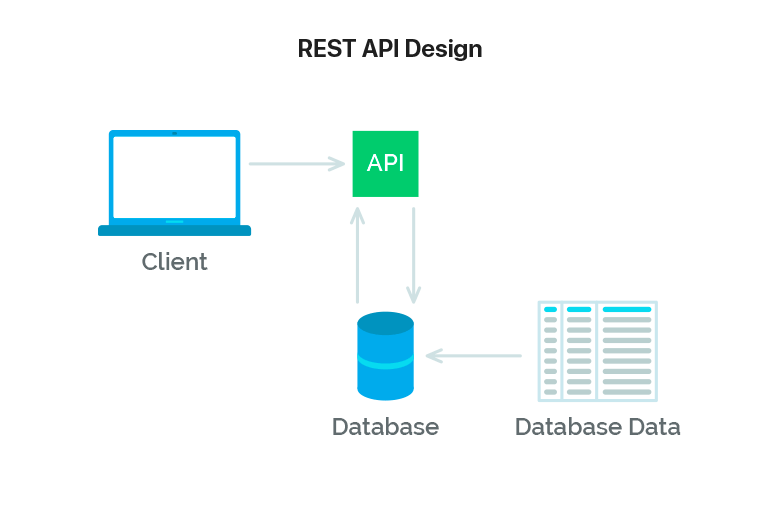
\includegraphics[width=0.8\textwidth]{REST}
\end{center}
The advantages of this architecture are:
\begin{itemize}
    \item Seperate the front end and back end. For us two person group, it is convenient that we can work on one
    without depending on the other.
    \item Allows us to run both ends at the same time.
    \item We can build and deploy both ends together or sepearated.
    \item Easy to use different tools on each end.
\end{itemize}
\textbf{Front-end web framework:} AngularJS\\[5pt]
AngularJS is a structural framework for dynamic web applications. It has following advantage:
\begin{itemize}
    \item It provides the capability to create single page application in a very clean and maintainable way. 
    \item It provides data binding capability to HTML. Thus, it gives user a rich and responsive experience.
    \item Views are pure html pages, and controllers written in JavaScript do the business processing.
\end{itemize}

\textbf{Back-end development:} Spring Boot and Spring Data JPA\\[5pt]
We used spring boot to provide the RESTful api that our frontend needed. Spring Data JPA is responsible 
for the data access layer, it provides an easy way to access the data in our database. With it we can mapping the 
data in our database to object that we can manipulate in Spring boot.\\[5pt]
It has following advantage:
\begin{itemize}
    \item It avoids writing lots of boilerplate Code, Annotations and XML Configuration.
    \item It reduces lots of development time and increases productivity.
    \item It provides Embedded HTTP servers like Tomcat, Jetty etc. to develop and test our web applications very easily.
    \item It provides lots of plugins to develop and test Spring Boot Applications very easily using Build Tools like Maven and Gradle
\end{itemize}
\textbf{DBMS:} MySQL\\[5pt]
We choose relational database(SQL) as our main storage. The reason is that our data is structural and 
well-formed, and many RDBMS have a good balance between durability and performance when doing ACID. 
For RDBMS, we choose MySQL which is the main database we learned so far. \\[5pt]
The schema will be introduced in the following section. We have 8 tables, 8 stored procedures, and 4 triggers.\\[5pt]
Procedures:
\begin{itemize}
    \item get\_games\_on\_date: get all games played on the given date, join 5 tables.
    \item get\_games\_given\_id: get a game's all information through, join 5 tables.
    \item get\_playes\_of\_team: get all playes in a team, join 2 tables.
    \item get\_team\_of\_player: get a player's team info, join 2 tables.
    \item get\_players\_given\_name: get all players whose name is like given name, used to search player
    \item get\_team\_game\_desc: get all team games in date descending way, join 2 tables.
    \item get\_player\_games\_given\_team\_and\_game: get player's stat in a game.
    \item get\_player\_game\_desc: get all player games in date descending way, join 2 tables.
\end{itemize}
Triggers:
\begin{itemize}
    \item update\_team\_season\_update: after update on team\_game, we need to update the average stats of a given team season.
    \item update\_team\_season\_before\_delete: before delete a team game, we need to update the win-loss info for a given team season.
    \item update\_team\_season\_delete: after delete a team game, we need to update the average stats of a given team season.
    \item update\_team\_game\_insert: after insert a game\_info, automatically insert two team game for awayTeam and homeTeam.
\end{itemize}

\section{Data Source}
We use \href{https://github.com/seemethere/nba_py}{NBA\_py} as our data source. It is a python client for NBA statistics located 
at stats.nba.com. 

\section{Conceptual Design}
\begin{center}
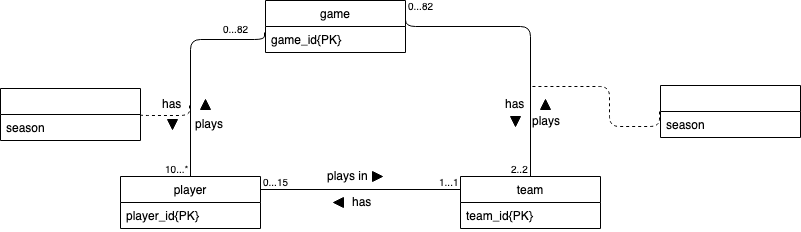
\includegraphics[width=1\textwidth]{CD}
\end{center}
For conceptual design, we can see that we have three main entities, game, player and team. Each team and player will play 0 to 82 games during a season, and one team will have 0 to 15 players, a player will belong to at most one team. During the game, there will be two teams, and no less than 10 players. Based on season and game, we can also derived the average stats of each team and player.
\section{Logical Design}
\begin{center}
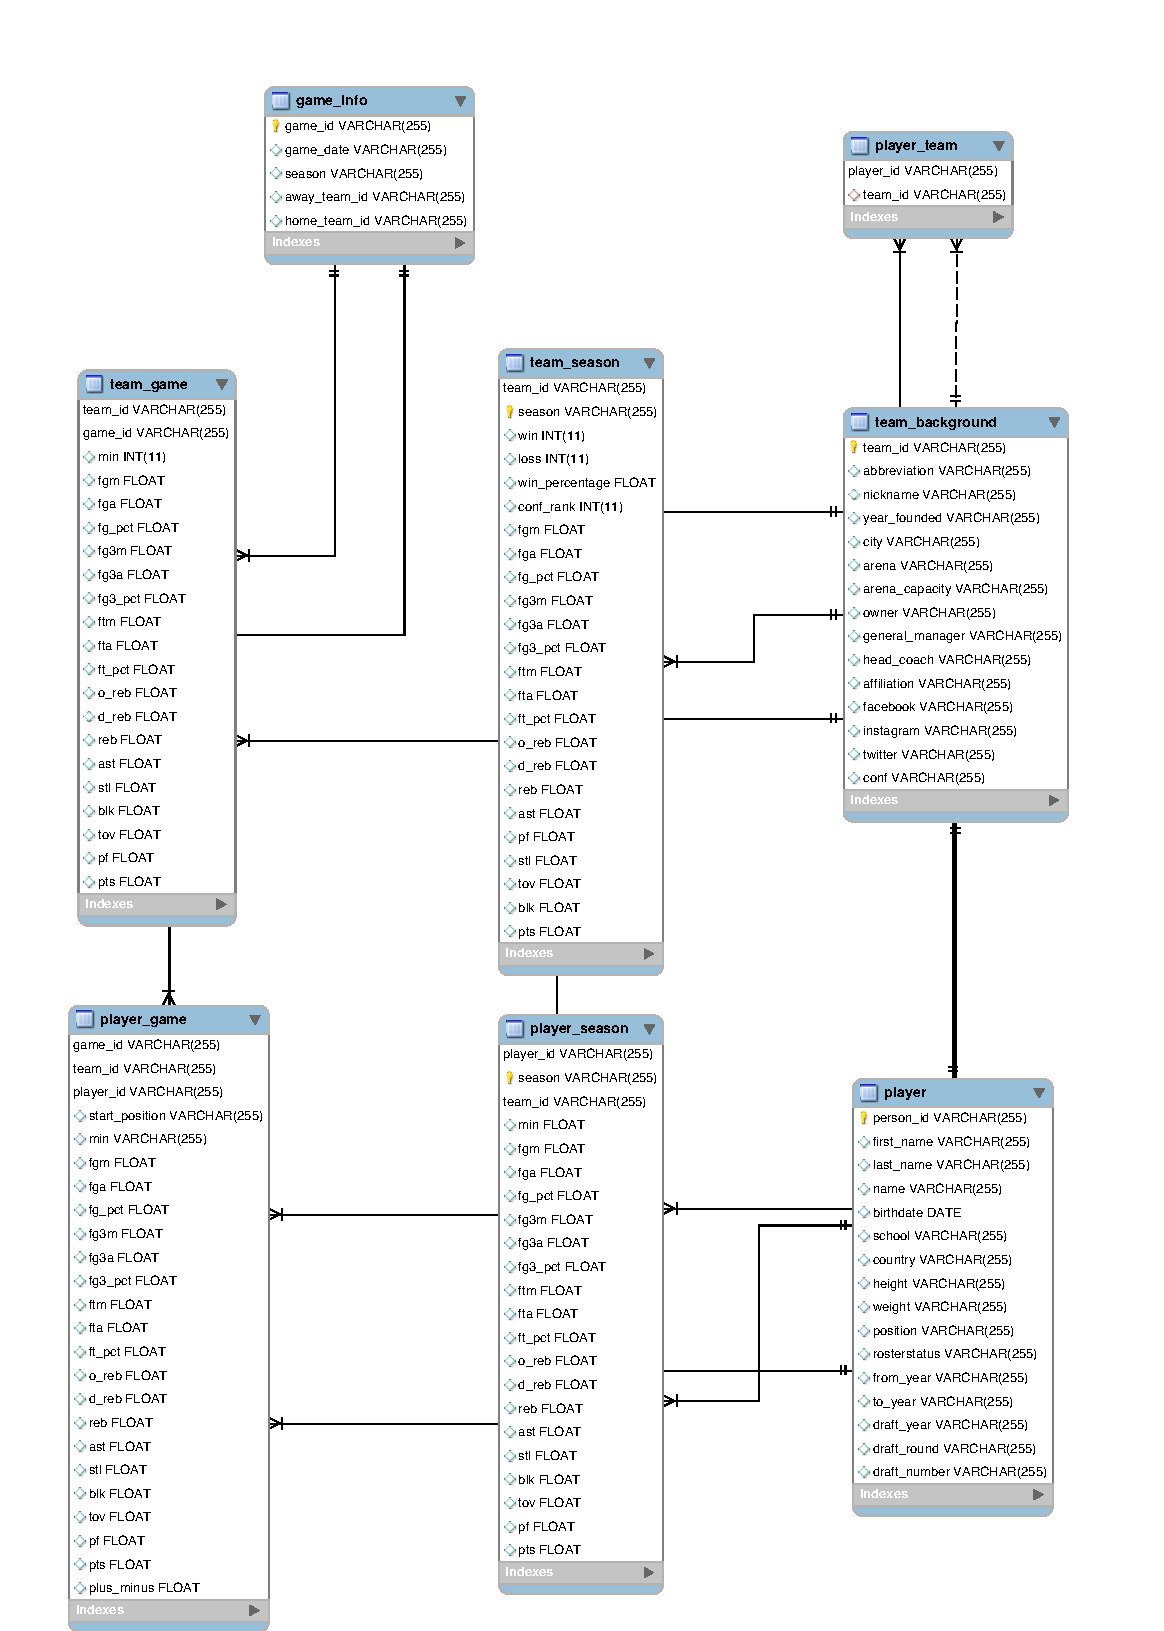
\includegraphics[width=1\textwidth]{schema}
\end{center}

\section{User flow}
\begin{center}
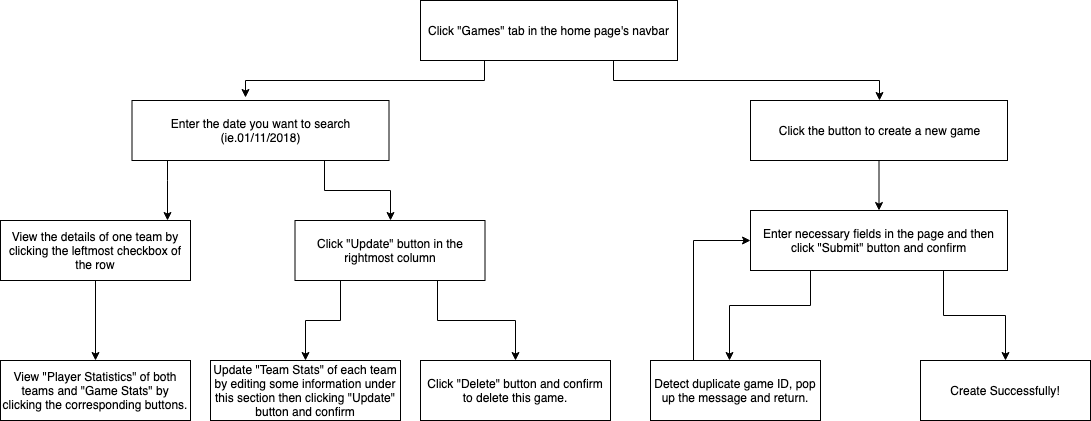
\includegraphics[width=1\textwidth]{User_Flow_Game}
Game flow
\end{center}

\bigskip
\begin{center}
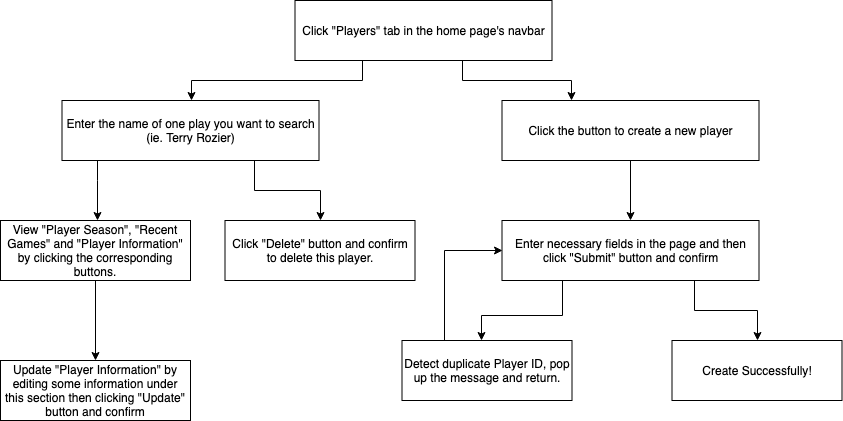
\includegraphics[width=1\textwidth]{User_Flow_Player}
Player flow
\end{center}
\bigskip
\begin{center}
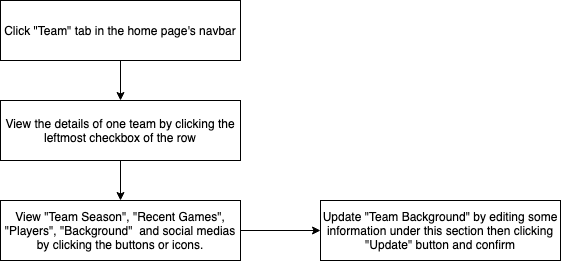
\includegraphics[width=1\textwidth]{User_Flow_Team}
Team flow
\end{center}

\section{Lessons Learned}
Technical expertise gained
\begin{itemize}
    \item Use python to fetch and preprocess data.
    \item Use springboot and spring data JPA to build a restful api.
    \item Use AngularJS to fetch data from http service and feed to HTML.
    \item Practice procedure, trigger we learned in course.
    \item Write complicated subquery.
\end{itemize}
Group work insights, time management insights, data domain insights
\begin{itemize}
    \item Good individual and group work. Seperating front end and back end makes the coorporation easier.
    \item Time management is flexible and not stressful as we start early.
    \item Data domain is not too complicated but the relationships between game, team and person need carefully think,
    as our table must follow 3rd and 4th norm.
\end{itemize}
Alternative design/approaches to the project
\begin{itemize}
    \item If we can use NoSql, we can store many other information type, including player picture, team picture. 
    \item Backend can use nodeJS and MongoDB, frontend can use Angular. Which is typically a MEAN stack. But this
    require more time for us to communicate as the application works as a whole.
\end{itemize}
Function not working
\begin{itemize}
    \item No function is not working. The data may lack because the player game data is too large and we don't have too much time
    to fetch and feed them into database. So we just download player games for two team in one season.
    \item We didn't implement insert player game, as one game will have more than 15 records, which will be a disaster for user 
    to type. So we only implement insert team game stats, our trigger will automatically update the team season after all.
    \item For data simplicity, we only import team game in season 2017-18.
\end{itemize}
\section{Future Work}
Planned uses of the database
\begin{itemize}
    \item This database can be provided to anyone who is interested in the data of NBA in season 2017-18. 
    \item People can do data analysis and visualization based on our databases. 
    \item Game developer may use our database to create new player, and create new game.
\end{itemize}
Potential areas of added functionality                                  
\begin{itemize}
\item Add the function of creating new team. 
\item Add more filters to query, like filter the player who can score 20+ and assist 5+.
\item Add some function to analyze the game, the player stats, maybe introducing some machine learning techiniques in our website.
\end{itemize}
\end{document}